\documentclass[11pt]{amsart}
\usepackage[margin=1.1in]{geometry}
\usepackage{amssymb,booktabs,url,graphicx}
\usepackage[hidelinks]{hyperref}

\newtheorem{theorem}{Theorem}
\renewcommand{\thetheorem}{\Alph{theorem}}
\newtheorem{corollary}[theorem]{Corollary}
\newtheorem{lemma}{Lemma}
\theoremstyle{remark}
\newtheorem*{remark}{Remark}

\newcommand{\Q}{\mathbb{Q}}
\newcommand{\p}{\mathfrak{p}}

\title[Class groups of exponent 7]{Imaginary quadratic fields with class group of exponent 7}
\author{Ben Gross}
\date{25 November 2026, revised 27 November 2026}
\subjclass[2020]{11R29 (primary); 11R11, 11Y40, 11M26}
\keywords{class group, exponent, imaginary quadratic field, generalized Riemann hypothesis, explicit formula, computer-assisted proof}

\begin{document}

\begin{abstract}\emergencystretch=1em
Assuming the generalized Riemann hypothesis for the quadratic Dirichlet $L$-functions of prime conductor, we show that exactly $33$ imaginary quadratic fields have class group of exponent $7$, with largest absolute discriminant $118843$. The proof does not use the earlier table of Elsenhans, Kl\"uners and Nicolae, which it recovers, or a published bound for the least split prime. With a result of Aiken, Ross, Shvydkoy and Xue it also shows that under ERH exactly $40$ imaginary quadratic orders have Picard group of exponent $7$. The proof also shows that for every prime $q\equiv3\pmod4$ with $q\ge3.1\cdot10^{20}$, the ideal class above the least split prime of $\Q(\sqrt{-q})$ has order at least $9$. The proof combines a positive-kernel explicit-formula certificate, checked in interval arithmetic, that bounds the least split prime, with a sieve search over the norm equation $4p^7=x^2+qy^2$. Large discriminants are excluded by one further certificate row and, beyond $2^{135}$, by a two-cell kernel with explicit Chebyshev estimates. Lean checks the two finite searches from $866$ per-prime certificates. In a shared Lean~4.35 build, the recently announced Dirichlet-GRH proof supplies the analytic hypothesis. The resulting theorem applies to every negative fundamental discriminant. All code, certificates, proofs and logs are public.
\end{abstract}

\maketitle

\section{Result}

For a negative fundamental discriminant $D$ write $E(D)$ for the exponent of the class group of $\Q(\sqrt D)$.

\begin{theorem}\label{thm:A}
Assume GRH for the Dirichlet $L$-functions $L(s,\chi_D)$ of the odd real primitive characters of prime conductor. Then no fundamental discriminant $D$ with $3.1\cdot10^{20}\le|D|\le10^{32}$ has $E(D)=7$.
\end{theorem}

\begin{corollary}\label{cor:B}
Assume ERH for the Dedekind zeta functions of the imaginary quadratic fields. Then exactly $40$ imaginary quadratic orders have Picard group of exponent $7$, the largest absolute discriminant being $118843$.
\end{corollary}

Corollary~\ref{cor:B} follows from Theorem~\ref{thm:A} and \cite[Theorem~1.3(6)]{ARSX}. Under ERH, the first two results below give the field count of Theorem~\ref{thm:E} from Theorem~\ref{thm:A} and the literature. Theorem~\ref{thm:E} itself uses neither of them.
\begin{itemize}
\item Elsenhans, Kl\"uners and Nicolae \cite[Theorem~1 and Table~1]{EKN}: the list of imaginary quadratic fields with $E(D)\le 8$ and $|D|\le 3.1\cdot10^{20}$ is complete. It contains $33$ fields of exponent $7$, with largest absolute discriminant $118843$.
\item \cite[Theorem~3]{EKN}, derived from Bach and Sorenson \cite{BS}: under ERH for the Dedekind zeta function of $\Q(\sqrt D)$ and for $|D|>e^{25}$, some prime $p\le(1.881\log|D|+6.18)^2$ splits in $\Q(\sqrt D)$. By Step~1 below a split prime forces $|D|\le4p^7$ when $E(D)=7$, so $E(D)=7$ requires $h(\log|D|)\ge0$, where $h(t)=\log4+14\log(1.881t+6.18)-t$. Since $h'(t)=14\cdot1.881/(1.881t+6.18)-1<0$ for $t>10.7$, $h$ is decreasing on $[\log10^{32},\infty)$. Since $\log10^{32}<74$, we have $1.881\log10^{32}+6.18<146$, and $4\cdot146^{14}=7998342040108832435319302324224<10^{32}$, so $h(\log10^{32})<0$. Hence no $D$ with $|D|\ge10^{32}$ has $E(D)=7$.
\item Aiken, Ross, Shvydkoy and Xue \cite[Theorem~1.3(6)]{ARSX}: under ERH, their table of $40$ orders of exponent $7$ is complete if no fundamental discriminant $D$ with $3.1\cdot10^{20}\le|D|\le3.9\cdot10^{30}$ has class group of exponent $7$. Theorem~\ref{thm:A} supplies this hypothesis.
\end{itemize}

The $33$ fields are $\Q(\sqrt{-q})$ for the primes $q={}$71, 151, 223, 251, 463, 467, 487, 587, 811, 827, 859, 1163, 1171, 1483, 1523, 1627, 1787, 1987, 2011, 2083, 2179, 2251, 2467, 2707, 3019, 3067, 3187, 3907, 4603, 5107, 5923, 63499 and 118843.
The class group is cyclic of order $7$, except for $q=63499$ and $q=118843$, where it is $C_7\times C_7$. The seven further orders of \cite[Table~A.7]{ARSX} are non-maximal, with discriminants $-f^2d$:
\begin{gather*}
-284=-2^2\cdot71,\qquad -604=-2^2\cdot151,\qquad -892=-2^2\cdot223,\qquad -1852=-2^2\cdot463,\\
-1948=-2^2\cdot487,\qquad -343=-7^2\cdot7,\qquad -1372=-14^2\cdot7.
\end{gather*}
Each has class number $7$.

The proof of Theorem~\ref{thm:A} uses the hypothesis $E(D)=7$ only for the prime ideals above the least split prime. It therefore gives a statement about every field in the range, whatever its class group.

\begin{corollary}\label{cor:C}
Assume GRH as in Theorem~\ref{thm:A}. Let $q\equiv3\pmod4$ be a prime with $q\ge3.1\cdot10^{20}$, let $p$ be the least prime that splits in $\Q(\sqrt{-q})$, and let $\p$ be a prime ideal above $p$. Then the ideal class of $\p$ has odd order at least $9$.
\end{corollary}

Finally, the same method applies below $3.1\cdot10^{20}$, and this removes the dependence of the field count on the table of \cite{EKN}.

\begin{theorem}\label{thm:D}
Assume GRH as in Theorem~\ref{thm:A}. Then exactly $33$ fundamental discriminants $D$ with $|D|\le10^{32}$ have $E(D)=7$, namely $D=-q$ for the $33$ primes $q$ listed above. This does not use \cite[Theorem~1]{EKN}.
\end{theorem}

Two further exclusions, under the same hypothesis, remove the bound $|D|\le10^{32}$ (Section~\ref{sec:E}).

\begin{theorem}\label{thm:E}
Assume GRH as in Theorem~\ref{thm:A}. Then exactly $33$ negative fundamental discriminants $D$ have $E(D)=7$, namely $D=-q$ for the $33$ primes $q$ listed above. This uses neither \cite[Theorem~1]{EKN} nor \cite[Theorem~3]{EKN}.
\end{theorem}

The integrated Lean theorem supplies the GRH premise of Theorem~\ref{thm:E} from the pinned formal proof in \cite{GRH}. Its statement retains the hypotheses that the discriminant is negative and fundamental. Section~\ref{sec:checks} identifies the Lean declaration and its inputs.

\subsection*{Context}
\cite[Theorem~2]{EKN} gives completeness under ERH for exponents $\le5$ and $8$. For exponents $6$ and $7$ the ERH bounds of \cite[Table~2]{EKN}, about $2.5\cdot10^{25}$ and $3.9\cdot10^{30}$, lie beyond their search limit, and \cite[Theorem~1.3(5),(6)]{ARSX} records both as conditional on these ranges. A computer-assisted note \cite{E6} treats exponent $6$ by a positive-kernel method that we adapt here. As \cite{EKN} remarks, at the time of their work finiteness of the list was known unconditionally for every exponent $2\le c\le 8$ except $c=7$.

\section{Proof of Theorem~\ref{thm:A}}

Let $D$ be fundamental with $E(D)=7$ and $3.1\cdot10^{20}\le|D|\le10^{32}$.

\subsection*{Step 0: genus theory}
The class group has odd order, so its $2$-rank, which is one less than the number of prime divisors of $D$, is $0$. Hence $D=-q$ with $q\equiv3\pmod4$ prime.

\subsection*{Step 1: the norm equation}
Let $p$ be a prime that splits, $(p)=\p\p'$. Then $\p^7=(\alpha)$ with $\alpha=(x+y\sqrt{-q})/2$, $x\equiv y\pmod 2$, and $y\ne0$, since otherwise $\p^7$ would be fixed by conjugation and equal $\p'^7$. Taking norms gives
\[
4p^7=x^2+qy^2,\qquad\text{so}\qquad q\le4p^7.
\]
Since $4\cdot691^7<3.1\cdot10^{20}$, no prime $p\le691$ splits. As $q>691$, these primes are inert; in particular $2$ is inert and $q\equiv3\pmod8$. Let $p$ be the least split prime. Then $p\ge701$ and every prime $\ell<p$ is inert.

\subsection*{Step 2: a split prime below an explicit bound}
Fix $X>2$ and a real step function $g$ on $[0,\log X]$ with $m=64$ cells of equal width. Let $f$ be its autocorrelation divided by $\int g^2$. Then $f$ is even and piecewise linear with nodes at multiples of the cell width, $f(0)=1$, $|f|\le1$, $f$ vanishes outside $[-\log X,\log X]$, and $\hat f=|\hat g|^2/\!\int g^2\ge0$.

Let $\chi=(-q/\cdot)$, an odd real primitive character of conductor $q$, and assume GRH for $L(s,\chi)$. The Guinand--Weil explicit formula (in the form of \cite[Lemma~9]{CMQR}) expresses $\sum_\gamma\hat f(\gamma)$, summed over the ordinates of the nontrivial zeros, as the archimedean and conductor terms minus the prime sum. Under GRH every $\gamma$ is real, so the left side is $\ge0$, and
\begin{equation}\label{eq:EF}
2\sum_{n<X}\frac{\Lambda(n)\chi(n)f(\log n)}{\sqrt n}\;\le\;\log\frac q\pi+\psi(3/4)+J_f,\qquad
J_f=\int_0^\infty\frac{2e^{-3u/2}}{1-e^{-2u}}\bigl(1-f(u)\bigr)\,du.
\end{equation}
Suppose no prime below $X$ splits. Since $q>X$ is the only ramified prime, every prime $p<X$ is inert, $\chi(p^k)=(-1)^k$, and the left side of \eqref{eq:EF} equals the explicit number
\[
\Sigma(X,g)=\sum_{p<X}A_p,\qquad A_p=2\log p\sum_{k\ge1,\;p^k<X}(-1)^k\,\frac{f(k\log p)}{p^{k/2}}.
\]
The kernel is chosen with $f$ negative on most of $(0,\log X)$, so that $\Sigma(X,g)$ is large and positive.
\begin{figure}[ht]
\centering
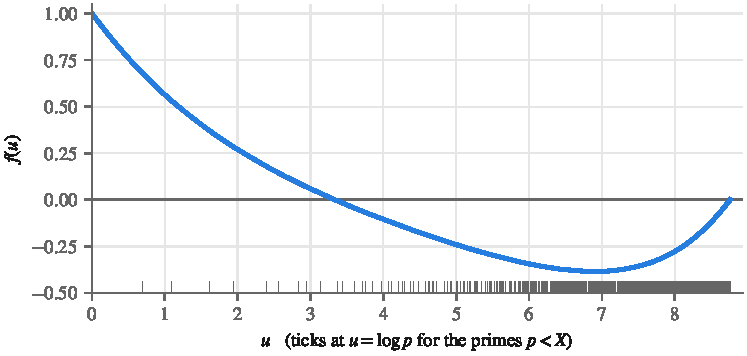
\includegraphics[width=0.74\linewidth]{fig_kernel.pdf}
\caption{The kernel $f$ of the first bootstrap row ($Q=10^{32}$, $X=6362$). Ticks mark $u=\log p$ for the primes $p<X$. Since $f(\log p)<0$ for all but the smallest primes, each inert prime contributes positively to $\Sigma(X,g)$.}
\label{fig:kernel}
\end{figure}
 A triple $(Q,X,g)$ is a \emph{valid row} if
\begin{equation}\label{eq:row}
\Sigma(X,g)-J^{+}-\log Q+\log\pi-\psi(3/4)>0
\end{equation}
for some $J^+\ge J_f$. By \eqref{eq:EF}, a valid row gives: every prime $q\equiv3\pmod 4$ with $X<q\le Q$ has a split prime below $X$.

\subsection*{Verification of the rows}
For each row the program \texttt{kernel\_verify.py} encloses every quantity in \eqref{eq:row} in outward-rounded intervals (\texttt{mpmath.iv}, $40$ digits). The autocorrelation values at the nodes are exact rationals, and the cell containing $\log n$ is determined by the exact integer comparison $X^k\le n^{m}<X^{k+1}$, so no floating-point step enters the verification. A second verifier, written independently in fixed-point integer arithmetic at scale $10^{-30}$ with its own series for $\log$ and $\exp$, accepts all $51$ rows with minimum margin $0.0126$. The margins are also proved in Lean (Section~\ref{sec:checks}). $J^+$ is obtained as follows. On the first cell we use $2e^{-3u/2}/(1-e^{-2u})=e^{-u/2}/\sinh u\le1/u$. On the other cells we split into $16$ subcells and use that the kernel is decreasing and $1-f\ge0$, so the kernel can be replaced by its value at the left end of each subcell. For $u>\log X$ the integral is bounded by $\tfrac43X^{-3/2}(1-X^{-2})^{-1}$. We use $\log\pi-\psi(3/4)=\log\pi+\gamma-\pi/2+3\log2$.

\subsection*{Step 3: bootstrap}
Six valid rows, each feeding $q\le4P^7$, with $P$ the largest prime below $X$, into the next:
\begin{center}
\begin{tabular}{rrrrr}
\toprule
$Q$ & $X$ & $P$ & margin $>$ & $4P^7$\\
\midrule
$10^{32}$ & 6362 & 6361 & 0.0126 & $1.686\cdot10^{27}$\\
$1.686\cdot10^{27}$ & 4690 & 4679 & 0.0160 & $1.964\cdot10^{26}$\\
$1.964\cdot10^{26}$ & 4393 & 4391 & 0.0188 & $1.259\cdot10^{26}$\\
$1.259\cdot10^{26}$ & 4333 & 4327 & 0.0191 & $1.136\cdot10^{26}$\\
$1.136\cdot10^{26}$ & 4319 & 4297 & 0.0181 & $1.082\cdot10^{26}$\\
$1.082\cdot10^{26}$ & 4312 & 4297 & 0.0147 & $1.082\cdot10^{26}$\\
\bottomrule
\end{tabular}
\end{center}
Hence $q\le4\cdot4297^7=108197560039107534049882852$, and the least split prime satisfies $701\le p\le4297$. A further $45$ valid rows $(Q_i,X_i)$, from $Q_i\approx8.1\cdot10^{25}$ down to $3.1\cdot10^{20}$, shorten the search: if $p\ge X_i$ then $q>Q_i$.
\begin{figure}[ht]
\centering
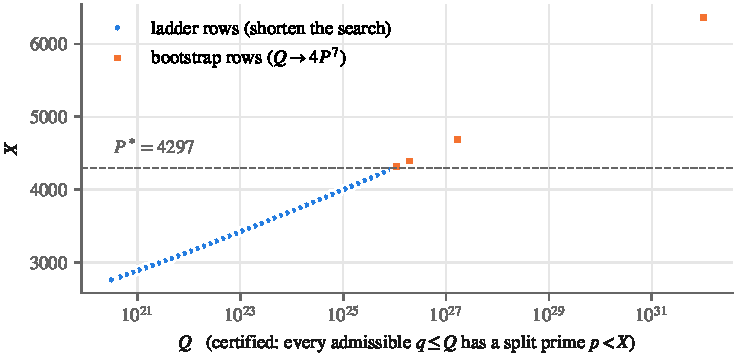
\includegraphics[width=0.74\linewidth]{fig_certificate.pdf}
\caption{All $51$ certificate rows. A row $(Q,X)$ certifies that every prime $q\equiv3\pmod4$ with $X<q\le Q$ has a split prime below $X$. The bootstrap rows (squares) reduce the range from $10^{32}$ to $4\cdot4297^7$. The ladder rows (dots) give each candidate $p$ a lower bound for $q$.}
\label{fig:certificate}
\end{figure}


\subsection*{Step 4: search}
For each of the $465$ primes $p\in[701,4297]$, each $y\ge1$, and each $x\ge0$ with $x^2\equiv4p^7\pmod{y^2}$ and $q=(4p^7-x^2)/y^2$ at least the lower bound given by the ladder for $p$, the program \texttt{sieve7} tests the necessary conditions $(-q/\ell)=-1$ for every odd prime $\ell<p$ and $q\equiv3\pmod8$. For $\ell\nmid y$ the first condition says that $x^2-4p^7$ is a non-residue modulo $\ell$, and this is sieved: a wheel on the first primes, $64$-bit residue patterns for $\ell<64$, then one prime at a time. In total there were $21{,}577$ arithmetic progressions, $7.8\cdot10^{12}$ positions after the wheel, $1.6\cdot10^{10}$ after the bit patterns, and no value of $x$ passing every odd prime $\ell<p$. So no such $q$ exists, and Theorem~\ref{thm:A} follows.\qed

\begin{figure}[ht]
\centering
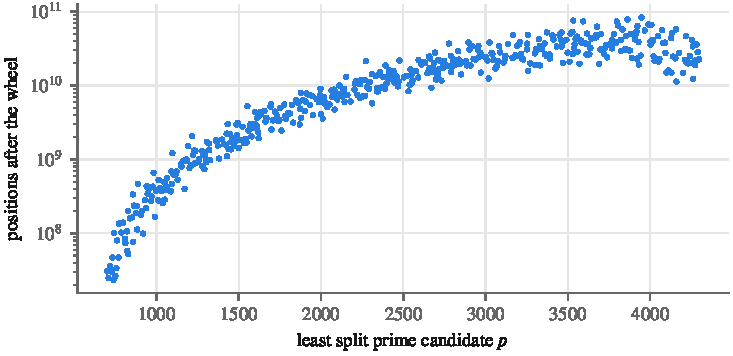
\includegraphics[width=0.74\linewidth]{fig_search.pdf}
\caption{Positions remaining after the wheel for each of the $465$ candidate primes $p$ in the production run. Every prime has $0$ survivors.}
\label{fig:search}
\end{figure}


\subsection*{Proof of Corollary~\ref{cor:C}}
Let $n$ be the order of the class of $\p$. The class number of $\Q(\sqrt{-q})$ is odd by genus theory, so $n$ is odd. As in Step~1, $\p^n=(\alpha)$ with $\alpha$ not rational, so $q\le4p^n$. If $q>10^{32}$, Section~\ref{sec:E} gives a split prime below some $X$ with $4X^7<q$, so $p<X$ and $n\le7$ would give $q\le4p^7<q$. Now let $q\le10^{32}$. By the first bootstrap row, $p\le6361$. If $n\le5$, then $q\le4\cdot6361^5<4.2\cdot10^{19}$, which is below $3.1\cdot10^{20}$. Suppose $n=7$. Steps~1 to~4 used $E(D)=7$ only to know that $\p^7$ is principal for the least split prime $p$: this gives $p\ge701$ in Step~1, it gives $q\le4P^7$ at each bootstrap row in Step~3 because the least split prime lies below $X$, and it gives the norm equation searched in Step~4. The search found no solution, so $n\ne7$. Hence $n\ge9$.\qed

\section{Proof of Theorem~\ref{thm:D}: the range below \texorpdfstring{$3.1\cdot10^{20}$}{3.1 x 10\string^20}}\label{sec:low}

By Step~0 and Theorem~\ref{thm:A} it suffices to find the primes $q\equiv3\pmod4$ with $q<3.1\cdot10^{20}$ whose class group has exponent $7$. Put $B=10^5$.

\subsection*{Below \texorpdfstring{$B$}{B}}
For each of the $4808$ primes $q\equiv3\pmod4$ below $B$ the class number is computed by counting reduced forms. It is a power of $7$ greater than $1$ for exactly $32$ of them. For $31$ it equals $7$. For $q=63499$ it equals $49$, and $\mathfrak l^7$ is principal for every split prime $\ell\le\sqrt{q/3}$, so the exponent is $7$. These are the $32$ listed primes other than $118843$.

\subsection*{More certificate rows}
The ladder is extended by $124$ valid rows $(Q_i,X_i)$, from $Q_i\approx2.3\cdot10^{20}$ down to $Q_i=B$, where $X_i=218$. Both verifiers accept all of them. Every row has $X_i<B$, so every row applies to every $q\ge B$.

\subsection*{The search}
Let $B\le q<3.1\cdot10^{20}$ with exponent $7$, and let $p$ be the least split prime. The row $(3.1\cdot10^{20},2760)$ gives $p<2760$, and $p\ne2$ because $4\cdot2^7<B$. So $2$ is inert and $q\equiv3\pmod8$. As before, $q$ exceeds $Q_i$ for every row with $X_i\le p$, and $4p^7=x^2+qy^2$ with $y\ge1$. Here $p\nmid y$: otherwise $p\mid x$, and then $p$ divides the generator $\alpha$ of $\p^7$, which is impossible because $\p'\nmid\p^7$.

A separate program, \texttt{lowsearch}, enumerates these solutions for the $401$ primes $3\le p<2760$. For each $y$ it computes the square roots of $4p^7$ modulo $y^2$ from the factorisation of $y$, by Tonelli--Shanks, Hensel lifting and the Chinese remainder theorem, and it checks every candidate exactly. It tested $2.83\cdot10^{12}$ candidates, with $y$ up to $1.1\cdot10^6$, and found $6608$ survivors $(p,x,y,q)$.

\subsection*{Classification of the survivors}
Of the $6608$ values of $q$, $4685$ are composite. For each of the $1923$ primes, reduction of the form of norm $p^7$ confirms independently that $\p^7$ is principal and that $p$ is the least split prime. For $1922$ of them the second split prime $\ell$ has $\mathfrak l^7$ not principal, so the exponent is not $7$. The remaining one is $q=118843$, found at $p=11$ with $(x,y)=(8128,10)$. Its class number is $49$ and its exponent is $7$. This proves Theorem~\ref{thm:D}.\qed

\subsection*{Checks}
\texttt{lowsearch} agrees with a brute-force reference on $106$ configurations, $105$ of them with survivors, including composite $y$ up to $659$. On the primes $701\le p\le760$, with the condition truncated to $\ell<60$, it produces the same $650{,}165$ survivors as the second implementation of Section~\ref{sec:checks}. The form-reduction test for principality agrees with the norm equation on $845$ small cases.

\section{Proof of Theorem~\ref{thm:E}: discriminants above \texorpdfstring{$10^{32}$}{10\string^32}}\label{sec:E}

By Theorem~\ref{thm:D} and Step~0 it suffices to show that no prime $q\equiv3\pmod4$ with $q\ge10^{32}$ has $E(-q)=7$. Both exclusions below are valid rows in the sense of \eqref{eq:row}. Each gives a split prime $p<X$ with $4X^7<q$, while Step~1 would give $q\le4p^7$.

\subsection*{The range \texorpdfstring{$10^{32}\le q\le2^{135}$}{10\string^32 <= q <= 2\string^135}}
Take $X=30000$ and the $64$-cell step function $g$ equal to $1$ on the first $32$ cells and to $-1$ on the last $32$. The kernel-checked evaluator of Section~\ref{sec:checks} certifies that $(2^{135},30000,g)$ is a valid row with margin at least $7.52277024130489382120$. A numerical evaluation using $J_f$ gives approximately $7.529$. Since $4\cdot30000^7<10^{32}$, the split prime furnished by this row satisfies $4p^7<q$.

\subsection*{The range \texorpdfstring{$q>2^{135}$}{q > 2\string^135}}
Take $g=[1,-1]$ on two cells of $[0,L]$, $L=\log X$. Then $f(u)=1-3u/L$ on $[0,L/2]$ and $f(u)=u/L-1$ on $[L/2,L]$, so $f<0$ on $(L/3,L)$. We use three facts.
\begin{enumerate}
\item $J_f\le4$ whenever $L\ge1$.
\item Put $Y=X^{1/3}$ and $w_T(t)=(1-\log t/\log T)/\sqrt t$. For every integer $X>1$,
\[
 B(X)=2\!\sum_{\sqrt X<p\le X} w_X(p)\log p
      -2\!\sum_{1\le n\le Y} w_Y(n)\Lambda(n)
      -\!\sum_{1\le d\le\sqrt X}\frac{\Lambda(d)}{d}
      \;\le\;\Sigma(X,g).
\]
The first sum runs over primes. On this interval $w_X(p)=-f(\log p)/\sqrt p$, accounting for the sign of an inert prime. The first subtracted sum bounds the negative contributions of the odd prime powers below $X^{1/3}$, where $f>0$, and the second those of the even prime powers, each paired with its square root; every other term of $\Sigma(X,g)$ is nonnegative.
\item For every $q>2^{135}$ there is an $n\ge19$ with $4\cdot2^{7n}<q$ and $\log q+4<B(2^n)$. This uses explicit lower and upper bounds for Chebyshev's functions and Abel summation.
\end{enumerate}
With $X=2^n$ from (3), facts (1) and (2), $\log\pi\ge0$ and $\psi(3/4)\le0$ make the margin of $(q,X,g)$ positive. For orientation, at $X=2^{19}$ a floating-point evaluation gives $\Sigma(X,g)-J_f+\log\pi-\psi(3/4)\approx381.51$, against $\log q\le142\log2\approx98.43$ at that dyadic index. The uniform estimate in (3) covers all larger indices.\qed

\section{Computation and checks}\label{sec:checks}

The production run took about $25$ minutes on $2$ virtual CPUs. A second run of the full search, on separate hardware with $26$ processes, produced identical output for every prime.

\subsection*{A second implementation}
A second search program, \texttt{search7i}, was written from the mathematical specification of Step~4 alone, without access to \texttt{sieve7} or its output. Its design is different. For each arithmetic progression $x=r+y^2k$ the value $q$ is a quadratic polynomial in $k$. The program enumerates the admissible residues of $k$ by a two-sided Chinese-remainder enumeration over $8$ and the small odd primes, filters the remaining candidates by table lookup over every odd prime $\ell<p$, and rechecks anything that passes in exact $128$-bit arithmetic. Before the full run it was compared with a brute-force reference on $240$ small configurations ($251{,}096$ survivors, all identical), and it recovers a solution of $4p^7=x^2+qy^2$ for each of the $28$ known fields of exponent $7$ with $q\equiv3\pmod8$. On the full range it took $111$ seconds on $24$ threads and found no survivors. For every one of the $465$ primes, its lower bound for $q$, its largest $y$ and its number of progressions agree with the production run.

\subsection*{A third implementation}
A third program, written by a different AI system (OpenAI's Codex) in an independent audit, lifts the admissible residues of $x$ directly modulo $8y^2$ and then by the Chinese remainder theorem over the small primes, combines further primes into periodic $64$-bit masks, and treats primes dividing $y$ on the exact value of $q$. It agrees exactly with a brute-force reference on $11$ windows and recovers all $33$ known fields. Its full run, reproduced on our hardware with identical totals ($77{,}049{,}566{,}290$ sieve blocks), finds no survivors. The same audit confirms from reduced forms that the two fields with class number $49$ have class group $C_7\times C_7$.

\subsection*{Further checks}
The following checks of \texttt{sieve7} are in the repository.
\begin{itemize}
\item \emph{Known fields.} For each of the $33$ known fields the class group is recomputed from reduced forms (exponent $7$ in every case; class number $7$, or $49$ for $q=63499$ and $118843$). A least split prime and a solution of $4p^7=x^2+qy^2$ are found, and the production code path of \texttt{sieve7} reports it.
\item \emph{Windows.} On $8$ windows, with the prime set truncated so that survivors exist, the survivor list is recomputed in Python from Jacobi symbols of $-q$ and agrees exactly with \texttt{sieve7}.
\item \emph{Fast versus naive.} $14$ runs comparing the wheel and bit-pattern path with a direct scan, $9$ of them with non-empty survivor lists, give identical lists.
\item \emph{Counts.} With truncated prime sets, the number of survivors over full $x$-ranges is compared with the product of local densities: $59{,}086$ found against $58{,}608$ expected over six runs, every survivor checked from the definition. A sieve that dropped candidates would show a deficit.
\item \emph{Source.} The exact source of the production binary is archived with its hash. The current source differs from it only by two test options whose defaults reproduce the production behaviour.
\end{itemize}

\subsection*{Formalization}
Theorems~\ref{thm:A}, \ref{thm:D} and~\ref{thm:E} are formalized in Lean~4 with Mathlib, in the directory \texttt{Exp7Lean} of the repository, with GRH as their only hypothesis. The statements use Mathlib's class group of the order $\mathbb Z[\omega]$, $\omega^2=b\omega+a$, of discriminant $D=b^2+4a$. The bounded declarations are \texttt{theoremA\_\allowbreak fundamental\_\allowbreak GRH} and \texttt{theoremD\_\allowbreak fundamental\_\allowbreak GRH}. Assume that for every prime $q\equiv3\pmod4$ every zero of $L(s,(\cdot/q))$ with $0<\operatorname{Re}s<1$ has real part $1/2$ (\texttt{GRHPrimeConductor}, stated for Mathlib's Dirichlet $L$-function), and let $D<0$ be a fundamental discriminant. If $3.1\cdot10^{20}\le|D|\le10^{32}$, the exponent of the class group is not $7$. If $|D|\le10^{32}$, the exponent is $7$ if and only if $D=-q$ for one of the $33$ listed primes $q$. The same equivalence without the bound on $|D|$ is \texttt{ChebyshevTail.\allowbreak classification\_\allowbreak fundamental}, which takes the two search statements as explicit arguments. The proofs \texttt{Exp7.searchHigh} and \texttt{Exp7.searchLow} supply them.

In Lean~4.35 the theorem \texttt{LFunction\_eq\_zero\_re} from the compact edition of \cite{GRH} supplies the project's GRH premise. The integrated theorem is
\begin{center}
\texttt{Exp7.GRHIntegration.theoremD\_fundamental\_global}.
\end{center}
It takes integers $a,b$ whose quadratic order is a domain with negative fundamental discriminant. The proof supplies GRH and both search certificates. The combined workspace applies compatibility patches to this project and has been built on one machine. The native project uses Lean~v4.37.0-rc1.

The completeness of the two searches is proved in Lean's kernel, from one certificate for each prime $p$. For the search of Step~4, the certificate lists, for each $y$, the residues of $x$ modulo $8y^2$ with a proof that the list is complete; each remaining arithmetic progression is cut into blocks, and the conditions $(-q/\ell)=-1$ are evaluated on packed bit vectors until the block is empty. For the search of Section~\ref{sec:low} the range of $q$ is cut in two. Below the cut the conditions on $q$ are periodic in $q$, and $q$ itself is sieved, which leaves an explicit list of exceptions. Above the cut $y$ is small, each $y$ is treated as in Step~4, and every surviving $x$ gives a $q$ that is among the $6608$ recorded survivors or violates one of the conditions. There are $465$ certificates for Step~4 and $401$ for Section~\ref{sec:low}; checking them takes about $11$ and $8$ core-hours. All $866$ certificates were also checked a second time, on a different machine and with a different version of Lean, by Codex.

\texttt{\#print axioms} reports only the three standard axioms (\texttt{propext}, \texttt{Quot.sound}, \texttt{Classical.\allowbreak choice}), and the development contains no \texttt{sorry} and no \texttt{native\_decide}: every computation is evaluated by the kernel. The other parts of the proof are formalized as follows: Step~0; Step~1, including $p\nmid y$; the explicit-formula inequality \eqref{eq:EF}, by a damped explicit formula, analytic continuation in the damping parameter, and Hadamard's partial fractions derived from Jensen's formula, without outside libraries; the closed form of $f$ and the bound $J^+$; the margins of all $176$ certificate rows, by a verified fixed-point evaluator run in the kernel; the tail above $2^{135}$; the bootstrap chain, the inert primes below $701$, the least split prime and its range, the Jacobi-symbol conditions and the ladder bounds; that the class group is generated by the prime ideals of norm at most $\sqrt{q/3}$; that each of the $33$ fields has exponent $7$; and, by tables checked in the kernel, that no other prime below $10^5$ and no other survivor of the search of Section~\ref{sec:low} does. The global proof uses the dyadic bound of Section~\ref{sec:E}. The count of $40$ orders in Corollary~\ref{cor:B} rests on \cite{ARSX} and is not formalized, and Corollary~\ref{cor:C} is not formalized.

\subsection*{Caveats}
Theorems~\ref{thm:A}, \ref{thm:D} and~\ref{thm:E} no longer rest on the search programs or on the numerical verifiers: the completeness of the searches and the margins of the certificate are proved in Lean. What remains to be trusted is Lean's kernel, including its arithmetic on large natural numbers, and the formal statements. A formal proof certifies the statements only as written, so the Lean statements of these theorems and the definitions they use (the class group, GRH, the list of $33$ primes) should be read by a person; they are short. The Lean development and the programs that generate the certificates were written by AI systems, and the paper has not been refereed. The statement for non-maximal orders rests on \cite{ARSX}. With the GRH premise discharged, Theorem~\ref{thm:E} rests on the formal proof of GRH of \cite{GRH}, which has been checked by machine but not refereed.

\subsection*{Data availability}
Earlier releases are archived on Zenodo. The merged global proof, its build instructions and the printed theorem statements are in the GitHub repository at commit \href{https://github.com/bgross0/exponent-seven/tree/99a97e077b9ddb2430d5da862a1d0842854330f1}{\texttt{99a97e0}}.
\begin{center}
\url{https://doi.org/10.5281/zenodo.24549331}\qquad \url{https://github.com/bgross0/exponent-seven}
\end{center}

\subsection*{Use of AI}
The argument, code and computations were produced with Claude (Anthropic) under the direction of the author, who takes responsibility for the content. The Lean formalization was produced with Claude; the packed bit-vector primitives used by the search certificates are due to ChatGPT (OpenAI). The independent audit, including the third search, the second certificate verifier and the second check of the Lean certificates, was produced with Codex (OpenAI). Codex also developed the finite bridge, the dyadic tail and their integration with the pinned GRH proof.

\begin{thebibliography}{9}
\bibitem{ARSX} D.~Aiken, E.~Ross, D.~Shvydkoy, H.~Xue, \emph{Boundary CM points and class groups of small exponent}, arXiv:2605.26020.
\bibitem{BS} E.~Bach, J.~Sorenson, \emph{Explicit bounds for primes in residue classes}, Math.\ Comp.\ \textbf{65} (1996), 1717--1735.
\bibitem{CMQR} E.~Carneiro, M.~B.~Milinovich, E.~Quesada-Herrera, A.~P.~Ramos, arXiv:2404.08380.
\bibitem{EKN} A.-S.~Elsenhans, J.~Kl\"uners, F.~Nicolae, \emph{Imaginary quadratic number fields with class groups of small exponent}, Acta Arith.\ \textbf{193} (2020), 217--233. arXiv:1803.02056.
\bibitem{GRH} L.~Alp\"oge, with Claude, \emph{Remark}, 20 November 2026, \url{https://alpo.ge/remark.pdf}. L.~Sernau and collaborators, shorter Lean formalization, compact edition (\texttt{grh-compact}), commit \texttt{72fead1}, \url{https://github.com/lsernau/grh-lean}.
\bibitem{E6} \emph{Class groups of exponent 6}, computer-assisted note, \url{https://github.com/nunavipahe60-star/exponent-six}, November 2026.
\end{thebibliography}

\end{document}
